\documentclass{article}
\usepackage{graphicx} % Required for inserting images
\graphicspath{ {./images/} }
\usepackage[letterpaper,top=2cm,bottom=2cm,left=3cm,right=3cm,marginparwidth=1.75cm]{geometry}
\usepackage{hyperref}

\begin{document}


\title{Unit 8 Learning Outcomes}
\author{Chris Hadden}
\date{}
\maketitle

\section{P1 Outline the tools available for digital marketing}

\subsection{What is Digital Marketing?}
The last couple of decades has seen a monumental shift in marketing, not only of internet brands like Google, but for all incumbent companies from super markets to estate agents.

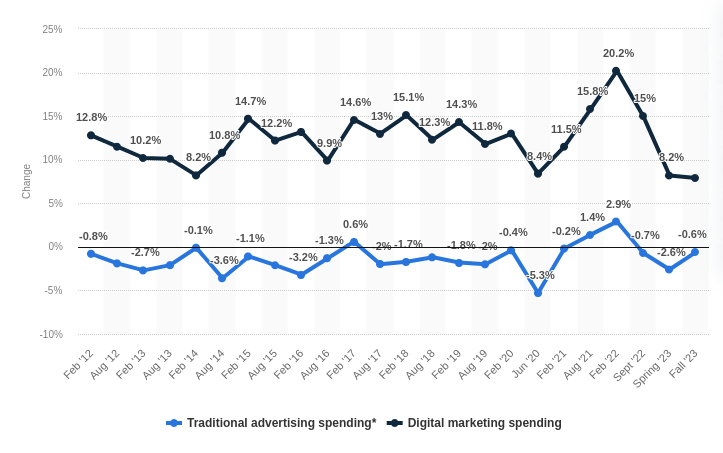
\includegraphics[scale=0.5]{TraditionalVsDigitalMarketing}

As you can see from this graph from Statista, from 2012 to 2023 in the US the spend on digital advertising had outstripped the spend on traditional advertising by a large margin. This is especially true during the Covid pandemic when most people were online a lot more.

The main advantages that digital marketing has is that 
\begin{itemize}
\item It is a lot cheaper thank buying slots on TV, etc
\item It is highly targeted, customers can be tracked and their buying habits monitored
\item It is easier to measure Return On Investment if you know who is looking at what adverts and what they are buying
\item It is personalised for greater effect
\end{itemize}

A modern digital marketing team will have many tools at their disposal, these would include the following

\subsubsection{Social Media}
There are a number of different types of Social media sites
\begin{itemize}
\item Sharing - Music, Video ,etc. Users can discuss shared media such as images and videos, this is a two way conversation and not like a mono user blog
\item Networking - Normally used to connect professional networks
\item Publishing - Can be used to publish blogs but can also be used to illustrate artwork, music, etc. These sites are useful as a self selection group meaning people on these specific sites are already interested in the exact media being shared there
\end{itemize}


\subsubsection{Email}
These days email is seen as a more traditional way to reach people but it is still very powerful.
An email may arrive in a personal inbox as text but can contain other digital artefacts such as pictures. Links can also be added to drive people to your site.

\subsubsection{Landing page optimisation}
A landing page is the initial page a user sees on your site.
The main techniques around optimising your landing page are
\begin{itemize}
\item Associative content targeting - the profile of the user changes the content they will see, such as geographical data, age, etc
\item Predictive content targeting - Using data about a users previous sales - Using algorithms it is possible to have a reasonable guess about what may interest a customer based on previous sales you know about. This can be hit or miss if you have a lot of products for sale
\item Consumer directed targeting - Responding to reviews from customers. If customers are responding that they do not like an item, it can be removed or updated
\item Closed end experimenting - Users are given options and they choose their favourite, for example different layouts of a page can be used to see which users like. This is A/B testing
\item Open ended experimentation - A final version of the page is never settled on, instead the landing page continues to develop and changes to match new users.
\end{itemize}

\subsubsection{Banners and popups/unders}
Banners are adverts that are seen, usually across the top of a webpage. The owner gets some money every time someone clicks on the advert. The advert will usually be presented from an advertising agency who will take a cut of the payment.
This is the closest method to traditional marketing as is mimics the layout of something like a newspaper.

The content of the advert can be tailored to the profile of the visitor.

Pop up and unders are adverts the open outside of the existing browser page. They are usually viewed as a bad thing as they are distracting and in many cases nefarious. Typically they are are seen to be used less and less on mainstream websites.

\subsubsection{SEO (search engine optimisation)}
Search Engine Optimisation is a massive area of research that continues since Google invented PageRank which ranked pages from a users search based on how useful Google thought the page was.
Research indicates that users will typically only look at the top search results so it's important to setup your site so it has the greatest change of being at the top of searches for what you are selling.

Many industries have been setup over the years to do SEO for websites, but in general the rule of thumb has been that you must provide as much relevant metadata about your site to search engines, and try to get as many links from other sites to yours, as this is usually seen as a good sign to search engines.

\subsubsection{Paid and organic search results}

\subsubsection{Channels}
Channels are the flow of how your messages gets to the customer.

Search engines are a popular channel. Putting adverts in a search engine means results for specific searches mean you page will be at the top of those results. This means you are much more likely to the clicked on as the relevant result.
Other channels are social media where brands can interact with customers as people. This means your brand will get more likes and can become more popular organically. Social media sites will track this interaction making it easy for you to see how effective it is being.
Finally you can pay social media to promote your brand messages for you as well.


\section{P2 Explain the stages of the digital marketing life cycle}

Each digital marketing campaign will be different, but overall they will usually follow the same steps that come together to make an identifiable lifecycle.

\subsection{Setup}
Typically 3 months

This is where your campaign is set up. 
You will have social media put in place, emails, marketing and websites should also be investigated.
Essentially you want to start acquiring customers, be that by sending out emails, posting to social media site or setting up newsletters that people can sign up it.
This is also when baseline KPIs (Key Performance Metrics) and metrics are determined. This is what you will measure your data against to determine if your marketing has been a success.
You can also prepare search engines and see if you gain followers or gain brand mentions.
\subsection{Traction}
This will typically be up to six months.

At this point you should be ramping up your campaign. If you are doing your SEO work correctly then you will see your site rising up in the search engine results, you will see you email sign ups increasing and your socials will be taking off.
You will also hopefully have contact with some potential customers or leads.

\subsection{Positioning}
You will be now 10 to 15 months past your initial setup.

The positioning phase is when you have established yourself. You will have higher rankings in search engines and competitors will be aware of your brand and products. 
You should also at this point have enough customers reaching out to you that you can derive metrics from them and be able to determine who they are and what it is they want from you. 

This stage is when you should be seeing a noticeable uptick in sales and customers are starting to express brand loyalty.
You should be seeing mentions of your products in blogs, social media outside your own, websites, etc.

\subsection{Expansion}
You are now at a point where you are over 16 months past your setup.

You position in your market has now galvanised. You are a well known player and can use this now clout to make better deals with customers and suppliers.

You should have stable and repeatable results from search results. You will still be using tools such as email marketing and socials but you will also have developed brand apps and maybe games. You will have social videos and brand ambassadors on many social media sites.

\subsection{Viral growth}
Viral growth is your ultimate goal.

Here you brand expands beyond what you can muster yourself as others start to spread the word of your brand and products.

Now your products will be in games, blogs, mobile, socials and even the news.



\break
\section{Sources}

\href{https://www.statista.com/statistics/693449/digital-vs-traditional-marketing-budget-change-according-to-cmos-usa/} {Traditional vs Digital marketing} \\

\end{document}

